\documentclass{article}

\usepackage[margin=2cm]{geometry}
\usepackage[latin1]{inputenc}
\usepackage{todo}
\usepackage{url}
\usepackage{caption}
\usepackage{subcaption}
\usepackage{graphicx}

\title{Fractal Drums}

\author{Knut Andre G. Prestsveen}

\begin{document}
\maketitle

\section{Abstract}
A numerical study of vibrations of fractal shaped drums. The 10 lowest vibration eigenmodes for a drum with a   fractal shaped boundary were computed using finite diferences, and the scaling of the integrated density of states were compared with the Weyl-conjecture and results for drums with smooth boundary.

\section{Introduction}
For any drum, it's size is related to the pitch of the sound it makes, and the larger the area, the lower the pitch. The question in mind for this study, is if the shape of the drum also affects the tone so that information about the drum's shape can be inferred from the tone, and this study spesifically studied drums shaped like quadratic Koch fractals.

The study was carried out numerically, and program code for generating the fractal and a system lattice, representing the drums boundary and skin respectively, were written. The eigenmodes of the drums vibration were then computed with finite differences, and to see if the Weyl-conjecture could could be used to infer information about the fractal boundary, the integrated density of states of the fractal drum were compared to that of a drum with smooth boundary and same area.

\section{Theory}
\subsection{The Weyl-conjecture}
The shape of the drum cannot be completely inferred from it's sound alone, but some information can be extracted. Firstly the area of the drum $A$ can be found from

\begin{equation}
    \label{area}
    A = 4*\pi ...,
\end{equation}
where $N(\omega)$ is the integrated density of states (IDOS), i.e. the number of eigenfrequencies smaller than the frequency $\omega$. Also Hermann Weyl conjectured that the second term in the asymptotic of $N(\omega)$ gives the length of the drums perimeter $L$, so that

\begin{equation}
    \label{weyl-conjecture}
    N(\omega) = \frac{A}{4*\pi}...
\end{equation}
in the limit of large $\omega$. Equation \ref{weyl-conjecture} is the Weyl-conjecture for the IDOS, and is proven correct under the assumption of a smooth boundary. This study tries to see what happens when the boundary is fractal.

\subsection{Quadratic Koch Fractal}
The quadratic koch fractal 

\subsection{Finite Difference Approximation}
Five-point and nine-point stensil. Equations...

\section{Code}
Cool code snippets and text explaining the implementation.

\section{Results}
Cool plots, and hopefully something clever about IDOS (If I am able to compute something sensible).

\begin{figure}
    \begin{subfigure}{0.3\textwidth}
        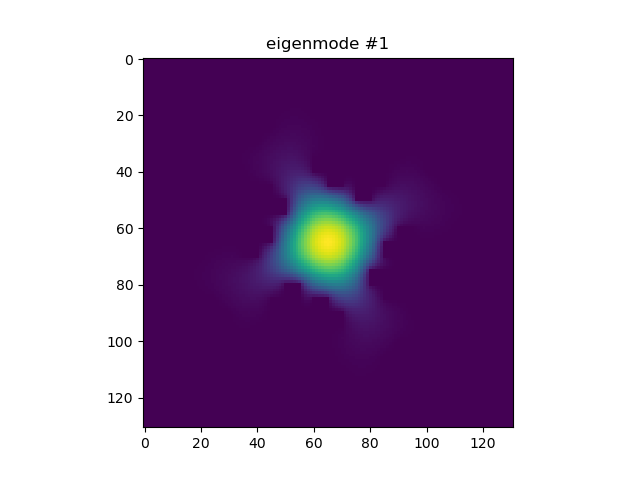
\includegraphics[width=\linewidth]{../figs/eigenmode_2d1.png}
    \end{subfigure}
    \begin{subfigure}{0.3\textwidth}
        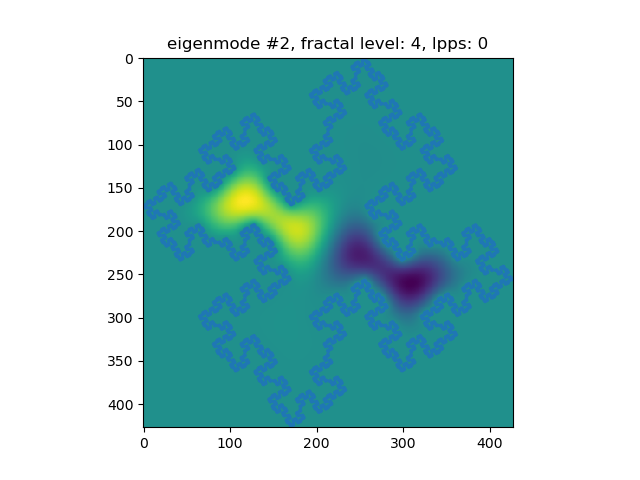
\includegraphics[width=\linewidth]{../figs/eigenmode_2d2.png}
    \end{subfigure}
    \begin{subfigure}{0.3\textwidth}
        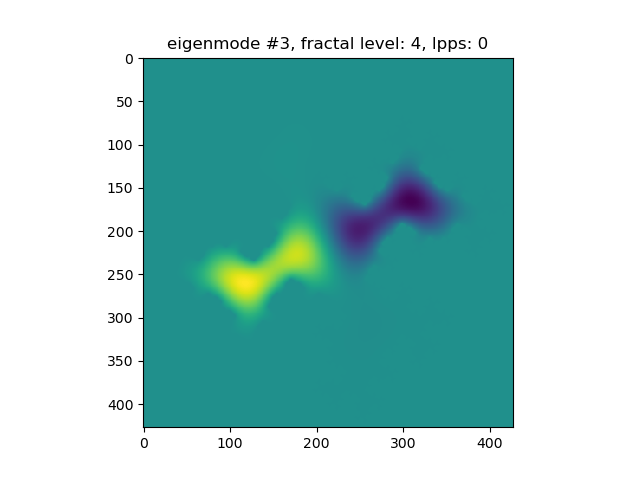
\includegraphics[width=\linewidth]{../figs/eigenmode_2d3.png}
    \end{subfigure}
    \begin{subfigure}{0.3\textwidth}
        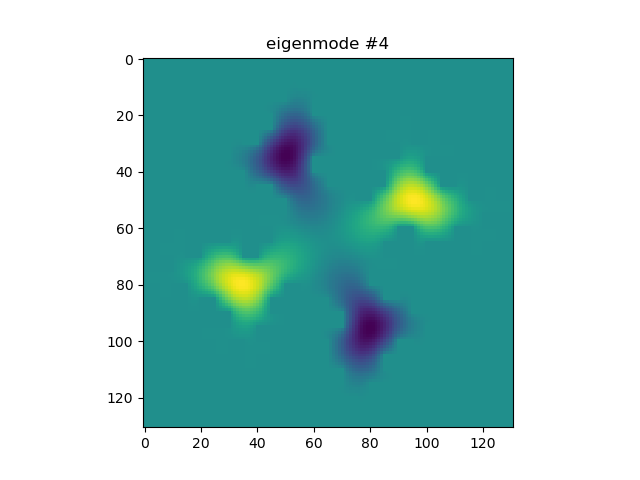
\includegraphics[width=\linewidth]{../figs/eigenmode_2d4.png}
    \end{subfigure}
    \begin{subfigure}{0.3\textwidth}
        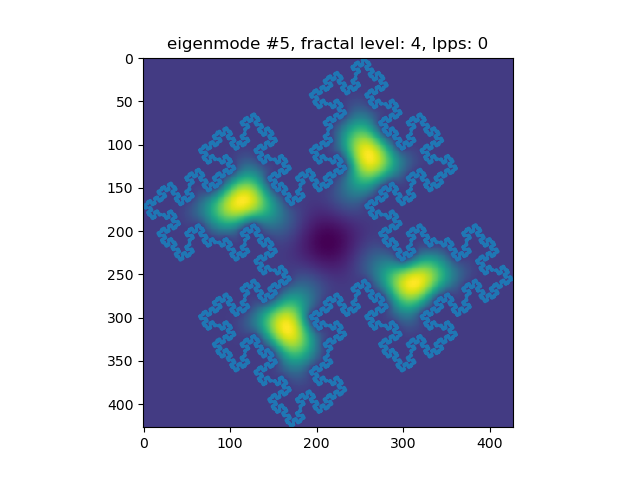
\includegraphics[width=\linewidth]{../figs/eigenmode_2d5.png}
    \end{subfigure}
    \begin{subfigure}{0.3\textwidth}
        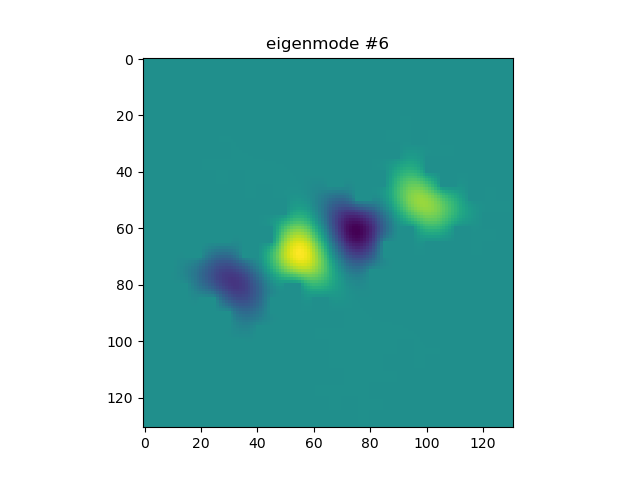
\includegraphics[width=\linewidth]{../figs/eigenmode_2d6.png}
    \end{subfigure}
    \begin{subfigure}{0.3\textwidth}
        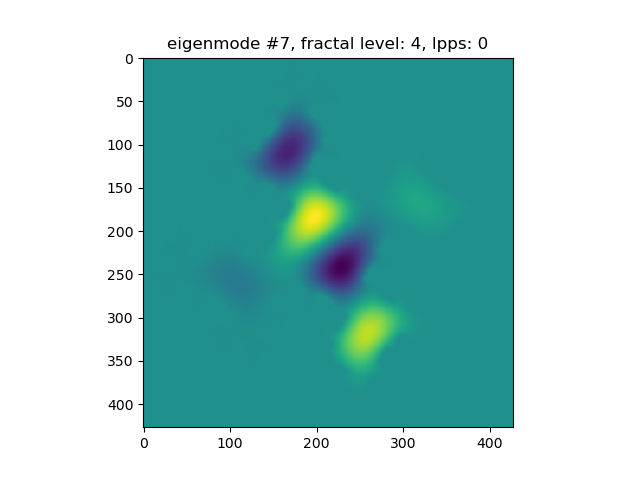
\includegraphics[width=\linewidth]{../figs/eigenmode_2d7.png}
    \end{subfigure}
    \begin{subfigure}{0.3\textwidth}
        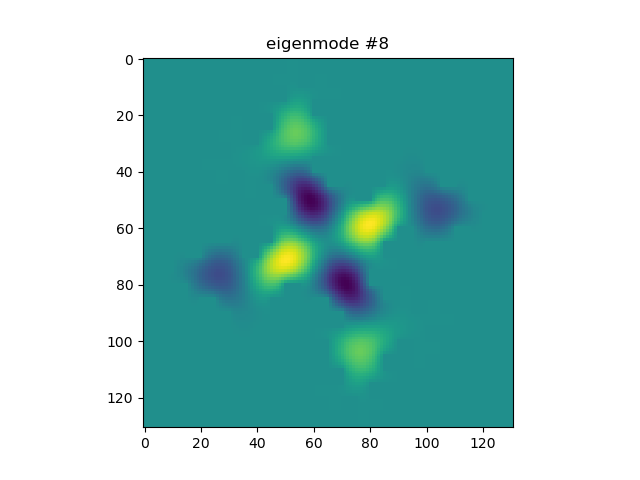
\includegraphics[width=\linewidth]{../figs/eigenmode_2d8.png}
    \end{subfigure}
    \begin{subfigure}{0.3\textwidth}
        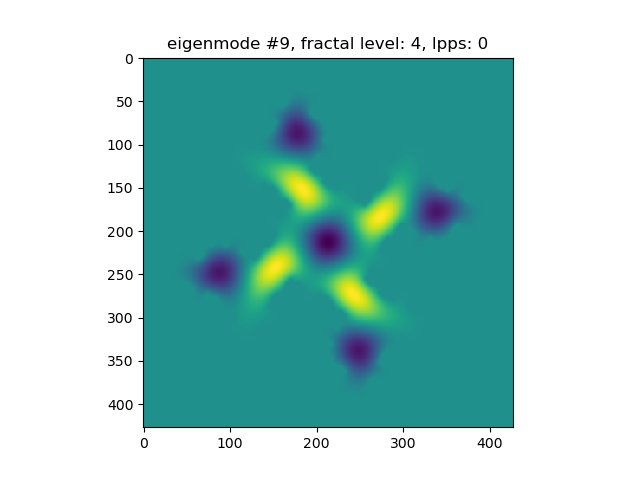
\includegraphics[width=\linewidth]{../figs/eigenmode_2d9.png}
    \end{subfigure}
    \begin{subfigure}{0.3\textwidth}
        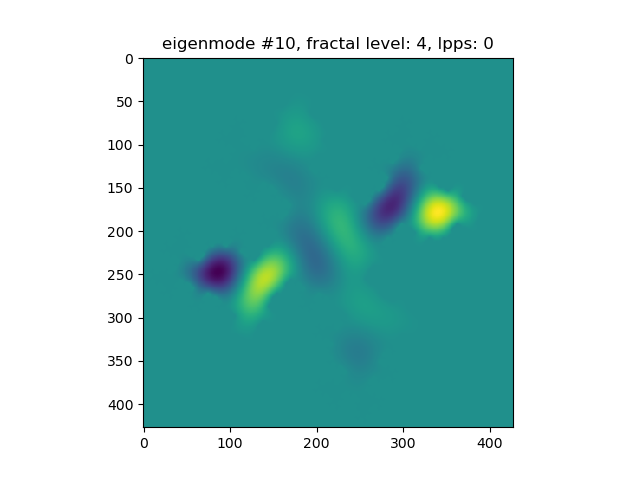
\includegraphics[width=\linewidth]{../figs/eigenmode_2d10.png}
    \end{subfigure}
    \caption{The 10 lowest eigenmodes, 2D plots.}
    \label{2dmodes}
\end{figure}

\begin{figure}
    \begin{subfigure}{0.3\textwidth}
        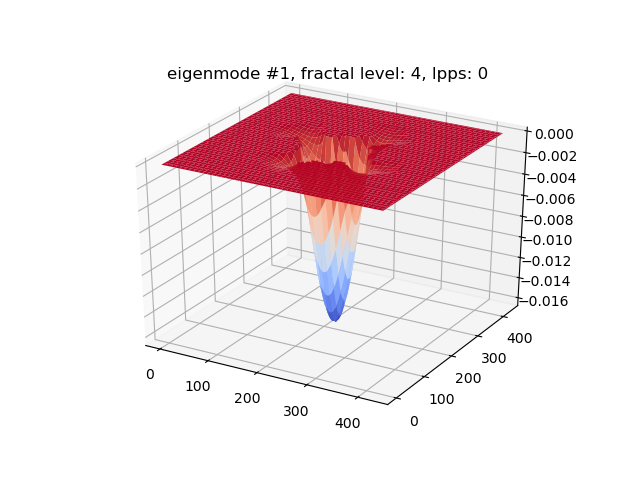
\includegraphics[width=\linewidth]{../figs/eigenmode_3d1.png}
    \end{subfigure}
    \begin{subfigure}{0.3\textwidth}
        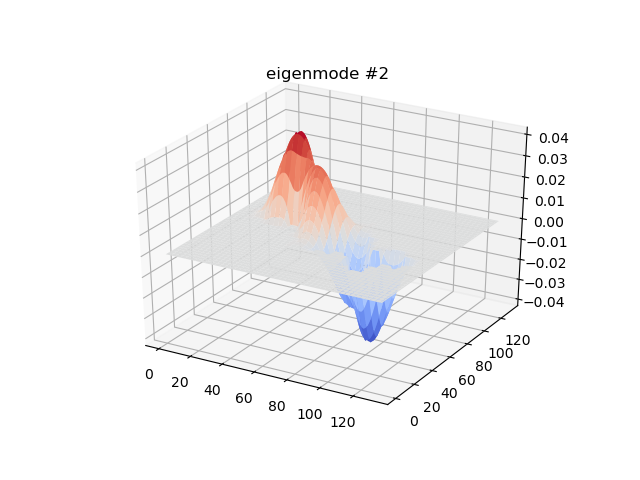
\includegraphics[width=\linewidth]{../figs/eigenmode_3d2.png}
    \end{subfigure}
    \begin{subfigure}{0.3\textwidth}
        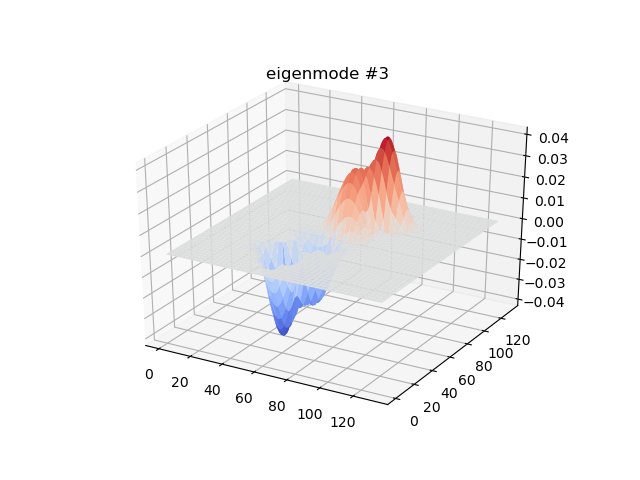
\includegraphics[width=\linewidth]{../figs/eigenmode_3d3.png}
    \end{subfigure}
    \begin{subfigure}{0.3\textwidth}
        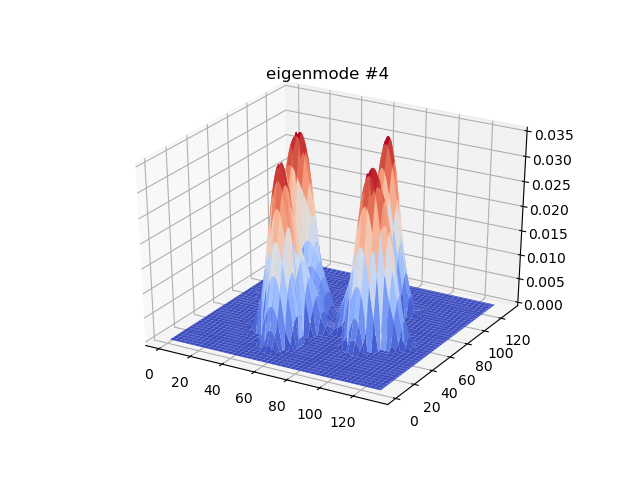
\includegraphics[width=\linewidth]{../figs/eigenmode_3d4.png}
    \end{subfigure}
    \begin{subfigure}{0.3\textwidth}
        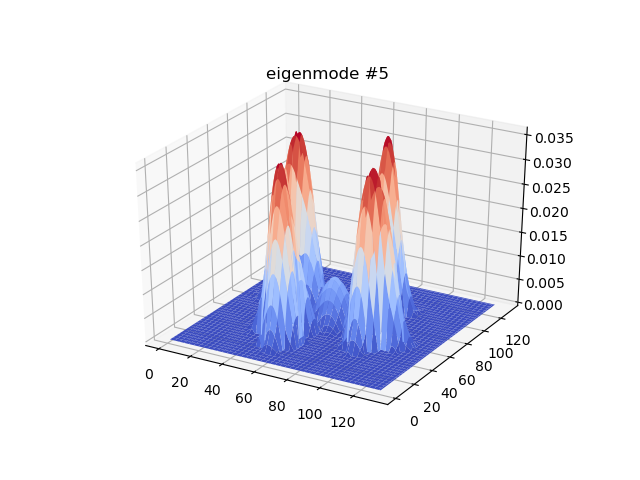
\includegraphics[width=\linewidth]{../figs/eigenmode_3d5.png}
    \end{subfigure}
    \begin{subfigure}{0.3\textwidth}
        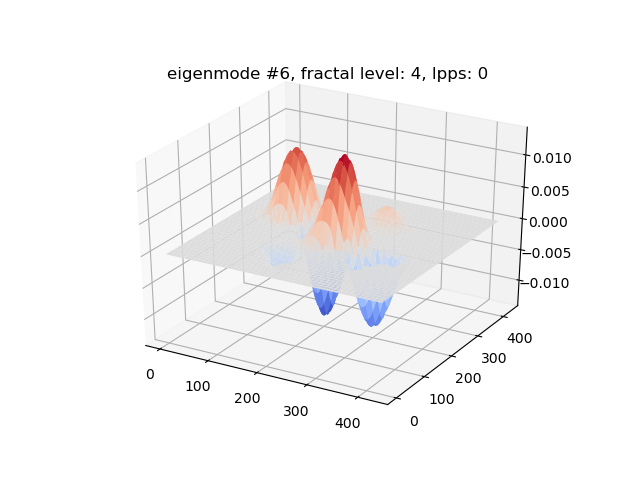
\includegraphics[width=\linewidth]{../figs/eigenmode_3d6.png}
    \end{subfigure}
    \begin{subfigure}{0.3\textwidth}
        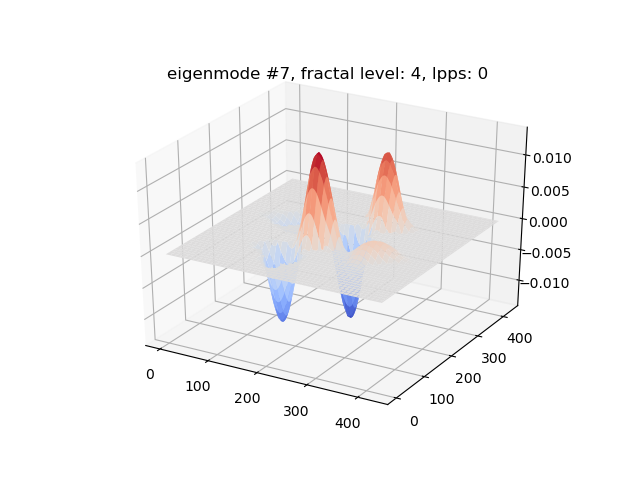
\includegraphics[width=\linewidth]{../figs/eigenmode_3d7.png}
    \end{subfigure}
    \begin{subfigure}{0.3\textwidth}
        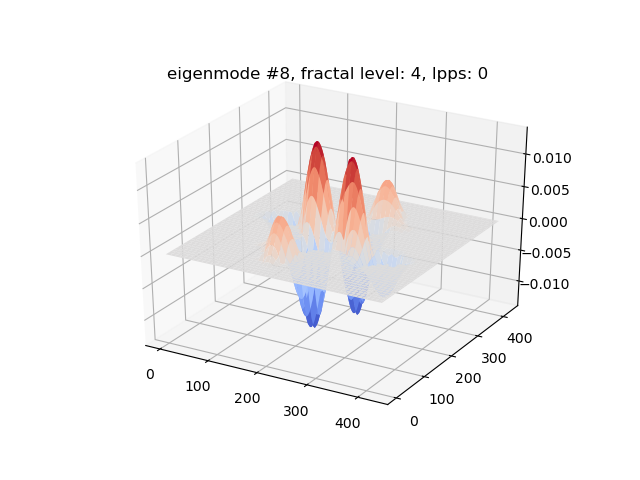
\includegraphics[width=\linewidth]{../figs/eigenmode_3d8.png}
    \end{subfigure}
    \begin{subfigure}{0.3\textwidth}
        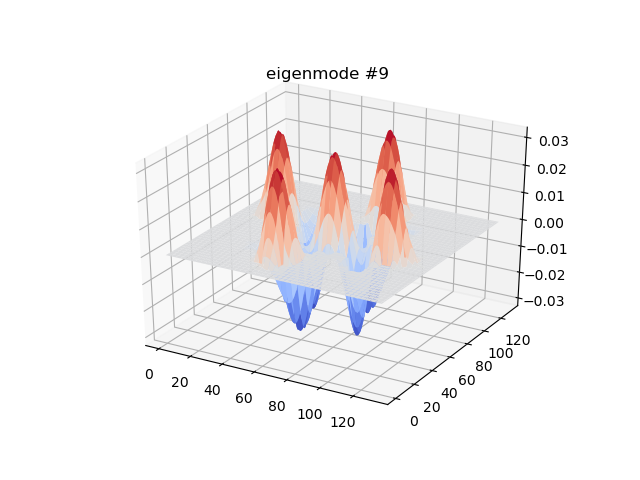
\includegraphics[width=\linewidth]{../figs/eigenmode_3d9.png}
    \end{subfigure}
    \begin{subfigure}{0.3\textwidth}
        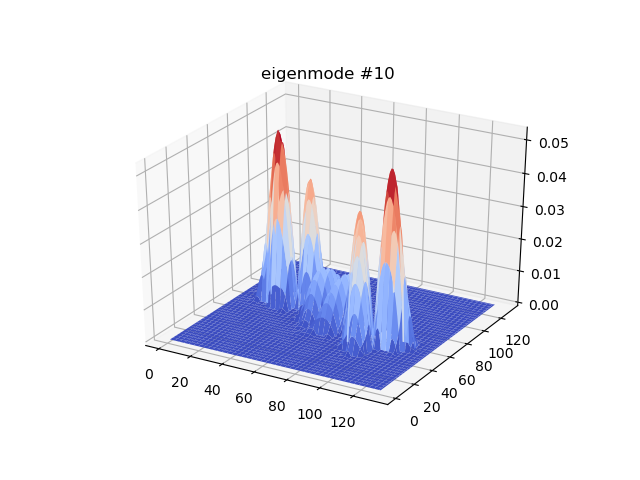
\includegraphics[width=\linewidth]{../figs/eigenmode_3d10.png}
    \end{subfigure}
    \caption{The 10 lowest eigenmodes, 3D plots.}
    \label{3dmodes}
\end{figure}

\end{document}

